\begin{frame}[fragile]{learning metrics}
\begin{align*}
%\phi & : \set X \to \set X ~~~~~ \text{learned from data}\\
d'_\phi(x,y) & = d(\phi(x),\phi(y))\\
\phi &= \argmin_{\phi} \sum_{(x,y) \in \mathcal X \times \mathcal X} \ell(x,y;\phi)
\end{align*}
%% image from: http://upload.wikimedia.org/wikipedia/commons/f/fd/Lle_hlle_swissroll.png
%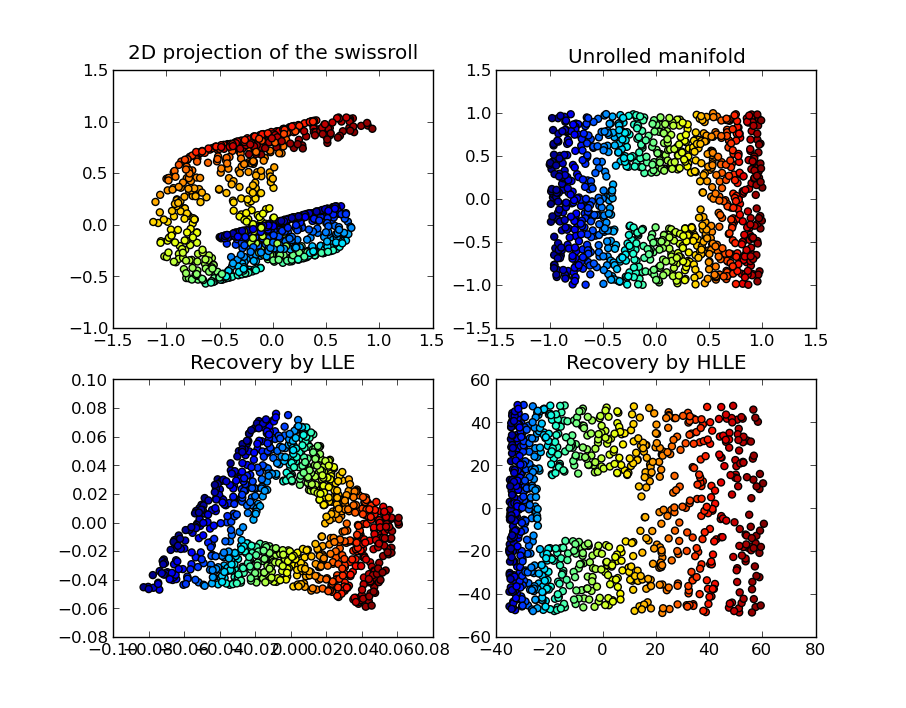
\includegraphics[height=9cm,width=12cm]{slides/covertree/swissroll.png}
% http://scikit-learn.org/0.12/_images/plot_compare_methods_11.png
\hspace{-1.5cm}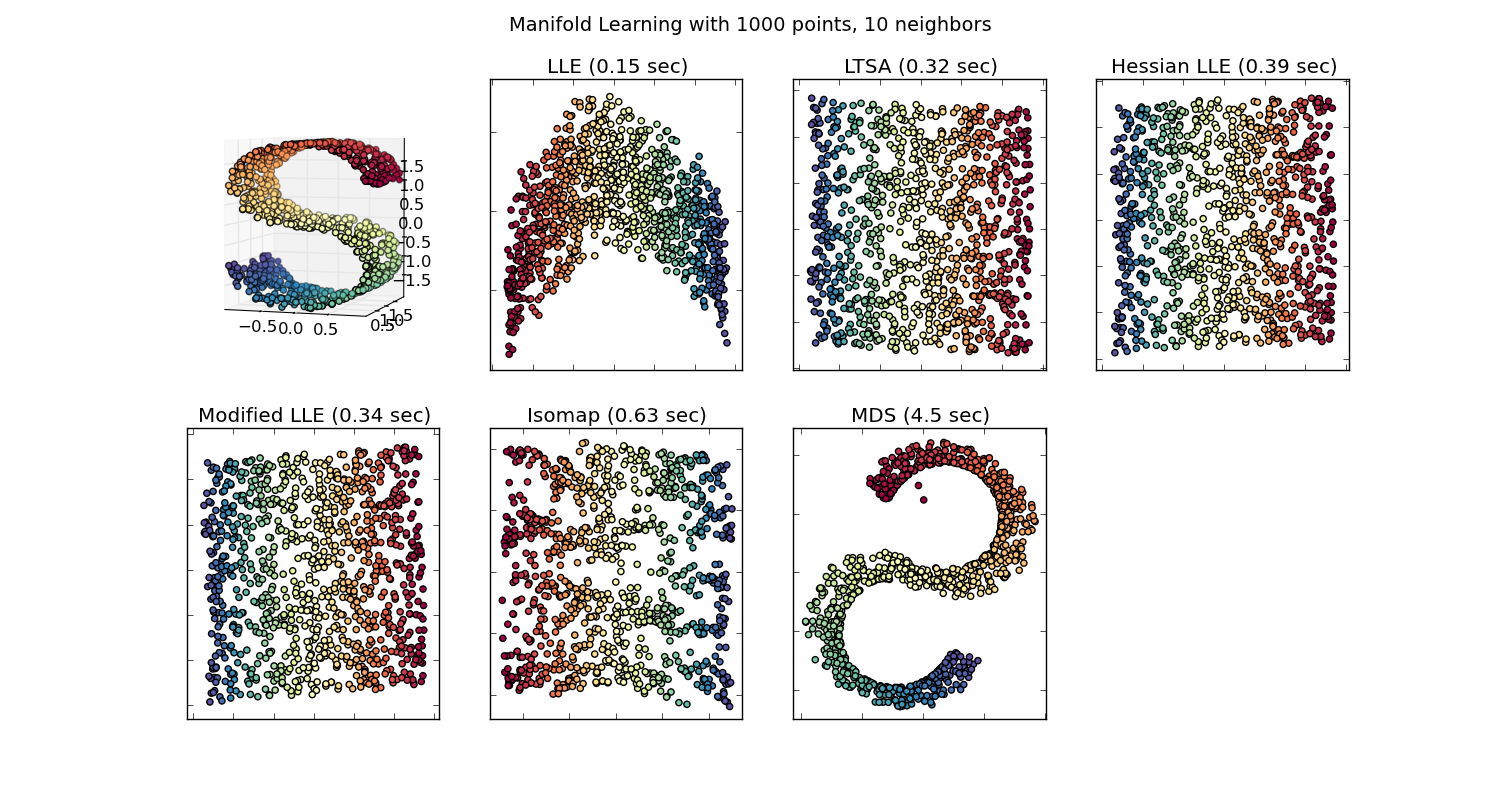
\includegraphics[height=6cm,width=15cm]{slides/covertree/manifold.png}
\end{frame}

